
% Diese ist ein Template zum Erstellen der Protokoll zum Praktikum Ein standardisierter und optimierter Prozess zur Erschließung von digitalen Herbarbelegen
% Fachgebiet Elektrotechnik und Informationstechnik, Leibniz Universität Hannover 
% 30/05/2017
% Cailin Guan 

\documentclass[10pt,a4paper]{report}

%%%%%%%%%%%%%%%%%%%%%%%%%%%%%%%%%%%%%%%%%%%%%%%%%%%%%%
%% grnutzte Package
\usepackage{ragged2e}
\usepackage{epsfig}  
\usepackage[utf8]{inputenc}
\usepackage[ngerman]{babel}
\usepackage{titlesec}
\usepackage{graphicx}
\usepackage[style=numeric-comp,backend=biber]{biblatex}
\usepackage{csquotes}
%%%%%%%%%%%%%%%%%%%%%%%%%%%%%%%%%%%%%%%%%%%%%%%%%%%%%%
\addbibresource{MyBib.bib}

%% ein paar kleine Modifikationen am Format
\parindent0pt                        % erste Zeile eines Absatzes nicht einrcken
\parskip 1.5ex                       % Absatzabstand
\raggedbottom                        
\renewcommand{\baselinestretch}{1.3} % Zeilenabstand
%%%%%%%%%%%%%%%%%%%%%%%%%%%%%%%%%%%%%%%%%%%%%%%%%%%%%%
%%
\titleformat{\chapter}
{\normalfont\bfseries} % format
{}{0pt}{\large}           % before-code
\titleformat{\section}
{\normalfont\bfseries} % format
{\thesection}{1em}{}        
\titleformat{\subsection}
{\normalfont\bfseries}{\thesubsection}{1em}{}
\titlespacing{\chapter}{0pt}{-50pt}{0pt}  

%%%%%%%%%%%%%%%%%%%%%%%%%%%%%%%%%%%%%%%%%%%%%%%%%%%%%%

%% Title Page
\title{Praktikumsprotokoll}
\author{Cailin Guan}
\date{\today}

%%%%%%%%%%%%%%%%%%%%%%%%%%%%%%%%%%%%%%%%%%%%%%%%%%%%%%%
%% Hier beginnt dieses Doku
\begin{document}
\maketitle  
% Erklärung für dieses Praktikum
\chapter*{Erklärung}

Hiermit erkläre ich, dass ich die vorliegende Arbeit selbst andig und ohne fremde Hilfe verfasst, und dass nur die angegebenen Quellen und Hilfsmittel verwendet wurden. Die Arbeit wurde bischer in gleicher oder änhlicher Form keineranderen Prüfungsbehörde vorgelegt.\\

Hannover, 30. Mai 2017\\

\underline{\hspace{4.5cm}}\\
Unterschrift
% Inhaltsverzeichnis	
\tableofcontents  
 
\chapter{Einleitung}

Vom September 2014 bis Mai 2017 arbeite ich in Teilzeit(33\%) an der Hochschule Hannover im Forschungsprojekt \glqq Standard Daten Akquisitionsprozess \grqq, Abkürzung \glqq stanDAP-Herb \grqq mit Visual Studio und C/C++/C\#. Dazu gehört die Entwicklung automatisierter Erkennung von Handschriftlichen Herbar - Belegen. Unter der Berücksichtigung bestehender Datenbanksystem und die Entwicklung einer funktionalen webbasierten, anwendungsorientierten Bedienoberfläche. Meinen Aufgaben zählen die digitalen Bildverarbeitung mit OpenCV Bibliothek und Programmierung, z.B GUI Oberfläche zur Web-Lokal-Steuerung, Objekterkennung mit Features, Klassifikation von multiple Objekten, Maschine Learning und Datenanalysieren wie XML und Json.\\
Ich habe am \glqq 3+1\grqq Austausch- und Kooperationsprogramm der Hochschule Hannover und der Partner Zhejiang University of Science and Technology in Hangzhou teilgenommen, und kam im Rahmen dieses Programms im Herbst 2013 nach Deutschland und belegte im WS13/14 einige englischsprachige Veranstaltung. Meine Praktikum und Bachelorarbeit absolvierte ich in diesem Forschungsprojekt \glqq stanDAP\-Herb\grqq. Danach habe ich einen Chance von Prof. Dr. Karl-Heinz Steinke bekommen, in diesem Projekt weiter zu arbeiten.\\
Das Thema \glqq Bildverarbeitung\grqq interessiert mich seit erstem Besuchen der Vorlesung \glqq Digitale Bildverarbeitung\grqq. Deshalb freute ich mich sehr, als ich die Arbeitsstelle bekam, und ich so die Möglichkeit bekam, im Rahmen dieser Teilzeitbeschäftigung arbeite ich mit zwei andere Studenten im Team zusammen. Dabei habe ich Berufserfahrung gesammelt und selbstständiges, eigenverantwortliches Arbeiten gelernt.\\

\chapter{Rahmenbedingungen}
\section{Art,Inhalt und Umfang dem Thema}

Das Projekt gehört zu Forschungsprojekt, die Grund, warum es gemacht wird, lautet, bisher werden die Metadaten von Herbarbelegen manuell in Sammlungsdatenbanken eingegeben, aber zunehmend werden Bilderfassungsverfahren eingesetzt, die auch die Nachprüfbarkeit der online verfügbaren Metainformation sichern. Das Standardverfahren soll nun so weit wie möglich die manuelle Metadatenerfassung ersetzen oder ergänzen. Bildverarbeitungssoftware erkennt Objekte auf dem digitalisierten Herbarbeleg und klassifiziert sie. Die Textobjekte werden mit Hilfe von Text - Mining Algorithmen in strukturierte Information überführt. Bei Handschriften wird versucht, den Autor zu erkennen. Im Projekt wird vorhandene Software evaluiert, unter Bildung von standardisierten Interfaces weiterentwickelt und in eine übergreifende offene Softwarearchitektur auf Grundlage etablierter IT-Standards integriert. Abschließend wird das Verfahren hinsichtlich seiner Anforderungen als Standard formuliert und hinsichtlich seiner Anwendung dokumentiert. Das Verfahren adressiert einen großen Bereich naturwissenschaftlicher Sammlungen, allein in Deutschland liegen ca. 22 Millionen Herbarbelege vor, weltweit über 500 Mio \cite{1}.\\
\begin{figure}[htbp] 
	\centering
	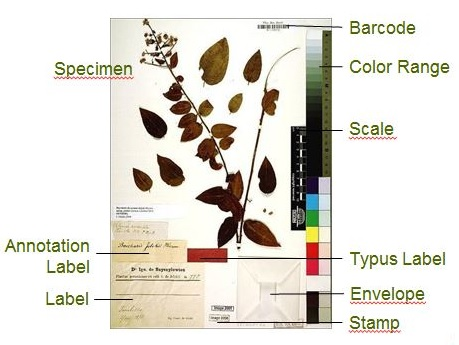
\includegraphics[width=0.7\textwidth]{Herbarbeleg_Objekte.JPG}
	\caption{Beispiel zu digitalem Bild \cite{2}, auf Herbarbelegen werden Metadaten wie Artname, Fundort und - datum, Sammler, Katalognummern etc. mit Etiketten, Barcodes usw. flächig sichtbar auf den Bogen gebracht und damit im Foto oder Scan abgebildet.}
	\label{fig:Bild1}
\end{figure}


\section{Vorstellung des Projekt: StanDAP-Herb}

Das Projekt, Standard Daten Akquisitionsprozess - Ein standardisierter und optimierter Prozess zur Erschließung von digitalen Herbarbelegen, ist durch DFG Deutsche Forschungsgemeinschaft, Literaturversorgung und Information / Erschließung und Digitalisierung gefördert, dauert insgesamt 3 Jahre lang, ab Juli 2014 bis Juni 2017. Das Ziel von diesem Projekt ist, einen softwarebasierten Standardprozess für die Extraktion von Metadaten von digitalen Herbarbelegen zu entwickeln und dokumentieren. Die Partnern von diesem Projekt sind \textit{Botanic Garden and Botanical Museum Berlin}, \textit{Fraunhofer IOSB - Karlsruhe} uns \textit{Hochschule Hannover}.

\chapter{Aufgaben der Tätigkeit}
\section{Aufgabenzuteilung}

Im Rahmen des Projekt werden die Aufgaben von vier Mitarbeiten geteilt, meine Tätigkeiten im Team sind eine GUI Oberfläche zu entwickeln, um die Bilder und Metadaten zu steuern, XML Daten von OmniPage OCR Software und zu analysieren und Json Daten von gefundenen Objekten zu erzeugen. Einen kleinen Server zu bauen, um Die Lerndateien automatisch auszuschneiden. Einen SVM Klassifizierung - Server für Multiple Objekte zu bauen, und das rotes Typus zu erkennen. Für ganze Server Hunderttausend Lernbilder zu sortieren.

\section{Aufgabenbeschreibung}

Für weitere Details von meinen täglichen Aufgaben werden in der folgenden Abschnitten genauer beschreibt. 

\subsection{Visual Studio 2008 \& 2010}

\subsection{OpenCV}

\subsection{GUI: Web-Lokal-Steuerung}

\subsection{XML-Analysierung}

\subsection{Fuzzy Search}

\subsection{Rest-Service}

\subsection{Auto-Cut}

\subsection{HSV Farbraume}

\subsection{Segmentierung}

\subsection{SVM-Klassifikator}

\subsection{Automatischer Objekterkennung}

\subsection{Json}

\chapter{Zusammenfassung}

\section{Erfahrungsgewinnen}

\section{Auswirkungen auf die eigene Berufsvorstellung}

\section{Bewertung der eigenen Leistungen}

\section{Rückmeldung des Arbeitgebers}

\section{Zusammenfassung der Tätigkeit}

%\chapter{Referenz}
\printbibliography
	                      	
\end{document}   